\documentclass[10pt]{article}
\usepackage{graphicx,amssymb, amstext, amsmath, epstopdf, booktabs, verbatim, gensymb, geometry, appendix, natbib, lmodern}
\geometry{letterpaper}
%\usepackage{garamond}

\newcommand*\Title{Rapport de stage de fin d'études}
\newcommand*\subtitle{Sécurité, CI \& développement Java}
\newcommand*\Date{\today}
\newcommand*\Author{Alexandre Léonardi}
\title{Rapport de stage de fin d'études}
\author{Alexandre Léonardi}
\date{\today}
%-----------------------------------------------------------

\usepackage{cpistuff/cpi} % This is what makes your document look like a cpi document.

\begin{document}

\begin{titlepage}
\maketitle
\end{titlepage}

\linespread{1.15} %Set standard document linespacing

\setcounter{tocdepth}{2}
\tableofcontents
\addtocontents{toc}{~\hfill\textbf{Page}\par}
\pagebreak
\section*{Introduction}
Développement Java et développement d'une solution d'analyse statique de sécurité : ce sont les deux principales branches de mon stage. Il s'agit pour partie de prendre part aux contrats en Java d'Alter Frame, l'entreprise qui m'accueille pour la durée du stage, et d'autre part d'intervenir sur un projet en interne visant à mettre en place une analyse de sécurité systématique des projets Web au-travers de pratiques de CI\cite{ci_wiki}\footnote{Continuous Integration ou intégration continue}. 

Ce sujet a l'avantage d'être ouvert et diversifié. Il me permet d'une part de travailler sur du pur développement et d'autre part de mettre en pratique la composante sécurité de la formation FSI\cite{fsi}\footnote{Fiabilité et sécurité informatique}, tout en découvrant les concepts de CI qui m'étaient jusque là étrangers, ainsi que des technologies qui vont de pair telles que Docker.

En pratique, un troisième pan viendra s'ajouter à mon sujet de stage : un audit technique pour un client d'Alter Frame souhaitant des pistes d'amélioration de son application, notamment en termes de qualité de code. 

À noter que, par discrétion à leur égard, les noms des clients d'Alter Frame ne seront pas mentionnés et seront effacés des captures d'écran que vous trouverez dans ce document. Il en ira de même pour les différents projets.
\pagebreak

\clearpage
\vspace*{\fill}
\begin{center}
\begin{minipage}{.6\textwidth}
\Huge Rapport de synthèse
\end{minipage}
\end{center}
\vfill % equivalent to \vspace{\fill}
\clearpage
\pagebreak

\section{Présentation d'Alter Solutions Engineering} 
Alter Solutions Engineering, et plus particulièrement sa filiale Alter Frame, est l'entreprise qui m'a accueilli pour la durée de mon stage de fin d'études, nous allons donc commencer par la présenter rapidement.

\subsection{Les subdivisions d'Alter Solutions Engineering et leurs secteurs d'activité}
Alter Solutions Engineering est une entreprise relativement jeune : elle a été créée en 2006 et, si elle n'entre plus maintenant dans la catégorie des PME en termes de nombre de collaborateurs, elle reste une structure de petite taille.

Le siège social de l'entreprise se trouve à Versailles et c'est là où travaille l'équipe de développement française dont je fais partie. En pratique, il s'agit de l'équipe de développement d'Alter Frame qui est une entité enfant d'Alter Solutions Engineering (cf. section~\ref{subsec:frame}).

Alter Solutions Engineering est une société de conseil en hautes technologies mais en pratique, elle est composée de trois filières qui ont chacune une spécialité bien distinctes (cf. graphique~\ref{fig:filiales}).
\begin{figure}
  \centering
  \caption{Alter Solutions Engineering et ses filiales}
  \label{fig:filiales}
  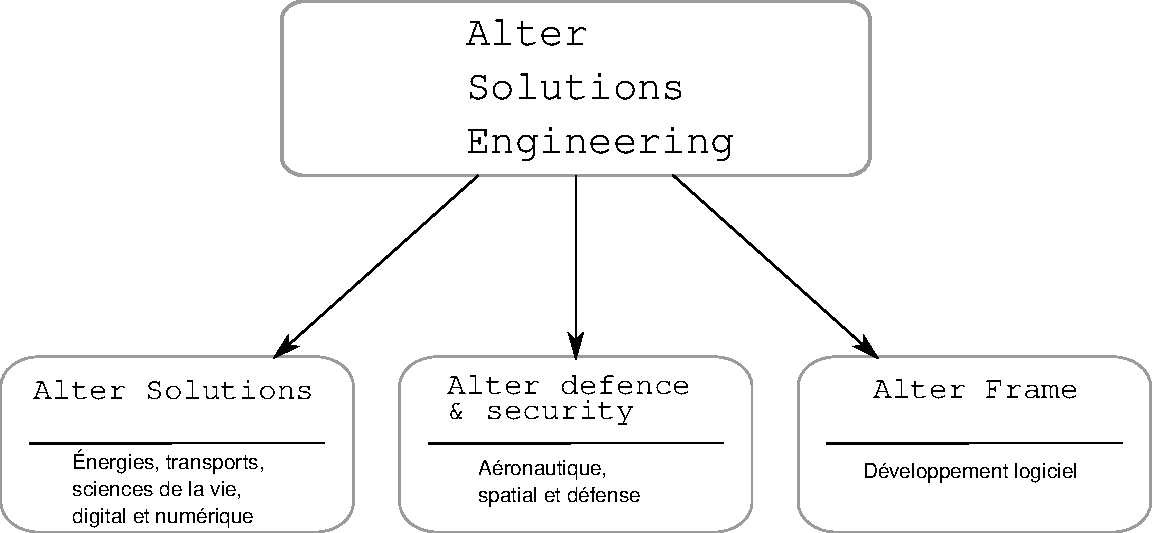
\includegraphics[width=\textwidth]{images/filiales_allinone.pdf}
\end{figure}

\subsubsection{Alter Solutions}
Cette filiale est spécialisée dans le conseil en ingénierie, notamment dans les domaines de l'énergie, des transports, des sciences de la vie, du digital et du numérique.

\subsubsection{Alter defence \& security}
Alter defence est également orientée vers le conseil, mais cette fois plus particulièrement dans l'aéronautique, le sptial et la défense.
  
\subsubsection{Alter Frame}
Alter Frame enfin est la branche spécialisée dans l'édition de logiciels et celle que j'ai rejoint durant mon stage. C'est une ESN\footnote{Entreprise de Services du Numérique, cf. \url{https://fr.wikipedia.org/wiki/Entreprise_de_services_du_num\%C3\%A9rique}} dont l'activité est elle-même répartie en deux catégories :
\begin{itemize}[label=$\bullet$]
\item le conseil, c'est-à-dire le fait de fournir des spécialistes d'un domaine du numérique pour la durée d'un contrat à un client ;
\item le développement de logiciels au forfait, c'est-à-dire le fait de prendre commande d'un logiciel à réaliser en interne et de le livrer à la fin du contrat.
\end{itemize}

\subsection{Un peu plus de détails sur Alter Frame}
\label{subsec:frame}
Bien qu'Alter Frame ait des clients et des domaines d'intervention variés, en termes de technologes il y a trois pôles de compétences qui sont caractéristiques de l'entreprise et reviennent le plus régulièrement :
\begin{itemize}[label=$\bullet$]
\item Java ;
\item .NET ;
\item PHP.
\end{itemize}

Mon stage ne s'est pas cantonné au domaine du développement mais il en a tout de même inclus celui-ci s'est déroulé au sein de l'équipe Java.
    
\subsection{Quelques (derniers) chiffres}
TODO : À remettre en forme pour plus tard
Mettre une note\footnote{\url{http://www.alter-solutions.com/notre-societe/chiffres-cles/}}.
375 collaborateurs en France, Portugal et Belgique (combien dans chaque pays ?)

\subsection{Répartition de l'activité}
\begin{tikzpicture}
    \pie[color ={ cyan!10 , cyan!20, cyan!30,  cyan!40}, explode=0.1]{10/A, 20/B, 30/C, 40/D}
\end{tikzpicture}

\pagebreak
\section{Retour d'expérience sur mon stage}
\pagebreak
\section{Environnement de travail \& solutions retenues}
Je ne suis intervenu que sur des projets qui étaient déjà commencés, et de ce fait il n'y a eu que peu de choix en termes de solutions retenues. Je vais néanmoins détailler ici l'environnement de travail, les différentes solutions techniques qui étaient déjà en place à mon arrivée et avec lesquelles j'ai travaillé pendant 6 mois.

Pour autant, il est intéressant de résumer l'environnement dans lequel j'ai évolué pendant 6 mois, pour chacun des pans très variés sur lesquels je suis intervenu. Les sous-sections seront volontairement brèves ; plus de détails seront disponibles dans les parties~\ref{sec:synthese_ci},~\ref{sec:synthese_java} et~\ref{sec:synthese_audit}.

\subsection{CI}
\subsubsection{GitLab \& GitLab-CI}
L'intégration continue dans les projets d'Alter Frame se fait à l'aide d'un service proposé par la plateforme d'hébergement de projets informatiques GitLab\cite{gitlab}. Le service en question, GitLab-CI\cite{gitlab-ci}, propose de mettre en place de l'intégration continue sur les projets hébergés sur GitLab.

Au moment de mon arrivée chez Alter Frame la partie CI des projets consistait majoritairement en la compilation des projets et une analyse de code à l'aide d'un plugin SonarQube\cite{sonarqube}, mise en place depuis environ 2 ans.

Le principe est que les actions décrites ci-dessus, compilation et analyse de code, sont effectuées à chaque push sur le serveur GitLab. Ce fonctionnement peut ensuite être affiné, pour ne se produire que lorsqu'un tag git est pushé ou sur certaines branches (branche master, tag de release, etc).

Il n'y avait néanmoins pas de composante cybersécurité dans le processus de CI d'Alter Frame et c'est donc ce sur quoi je suis intervenu en priorité. Néanmoins, mon travail ne s'est pas limité à cela et j'ai aussi pu intervenir sur d'autres aspects du CI et améliorer l'existant.

\subsubsection{ZAP : Zed Attack Proxy}
\begin{figure}
	{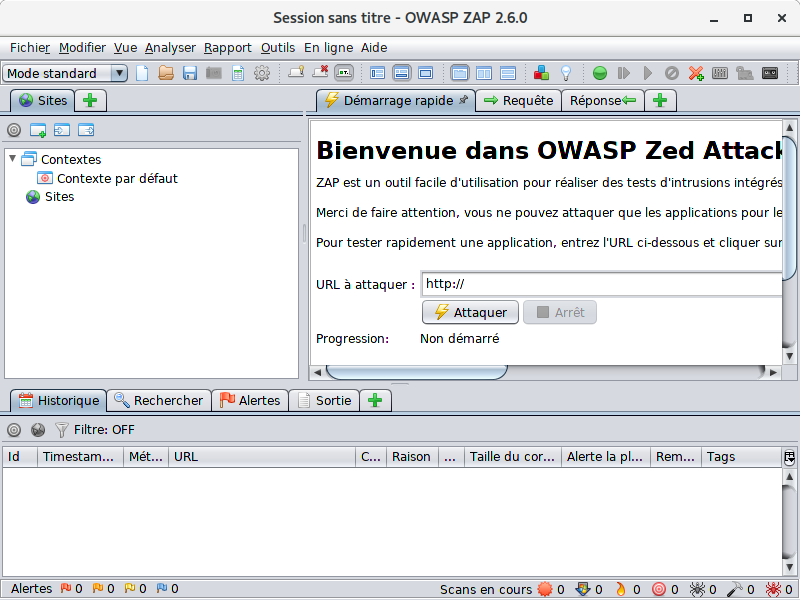
\includegraphics[width=\textwidth]{images/zap_acceuil}}
	\centering
	\caption{Fenêtre de démarrage de ZAP}
	\label{fig:zap_acceuil}
\end{figure}
ZAP\cite{zap} (voir figure~\ref{fig:zap_acceuil}) est un projet open source développé par l'OWASP\cite{owasp}. Il s'agit un proxy qui peut intercepter et analyse le trafic qui traverse la machine hôte. ZAP est un outil de sécurité très intéressant et ce pour un grand nombre de raisons :
\begin{itemize}[label=$\bullet$]
	\item activement développé\cite{zap_git} ;
	\item open source et cross-platform ;
	\item OWASP est une référence dans le monde de la sécurité ;
	\item une large communauté, et donc une grande quantité de ressources sur laquelle s'appuyer ;
	\item ZAP est contrôlable en ligne de commande (voir extrait~\ref{lst:zap_options}) et \textit{via} des APIs en plusieurs langages.
\end{itemize}

\begin{minipage}{\linewidth}
	\begin{lstlisting}[caption={Options de ZAP en ligne de commande},label={lst:zap_options},numbers=none]
$ zap.sh -cmd -help
Usage:
    zap.sh [Options]
Core options:
    -version                 Reports the ZAP version
    -cmd                     Run inline (exits when command line options complete)
    -daemon                  Starts ZAP in daemon mode, ie without a UI
    -config <kvpair>         Overrides the specified key=value pair in the configuration file
    -configfile <path>       Overrides the key=value pairs with those in the specified properties file
    -dir <dir>               Uses the specified directory instead of the default one
    -installdir <dir>        Overrides the code that detects where ZAP has been installed with the specified directory
    -h                       Shows all of the command line options available, including those added by add-ons
    -help                    The same as -h
    -newsession <path>       Creates a new session at the given location
    -session <path>          Opens the given session after starting ZAP
    -host <host>             Overrides the host used for proxying specified in the configuration file
    -port <port>             Overrides the port used for proxying specified in the configuration file
    -lowmem                  Use the database instead of memory as much as possible - this is still experimental
    -experimentaldb          Use the experimental generic database code, which is not surprisingly also still experimental
    -nostdout                Disables the default logging through standard output
Add-on options:
    -script <script>         Run the specified script from commandline or load in GUI
    -addoninstall <addon>    Install the specified add-on from the ZAP Marketplace
    -addoninstallall         Install all available add-ons from the ZAP Marketplace
    -addonuninstall <addon>  Uninstall the specified add-on
    -addonupdate             Update all changed add-ons from the ZAP Marketplace
    -addonlist               List all of the installed add-ons
    -quickurl [target url]: The URL to attack, eg http://www.example.com
    -quickout [output filename]: The file to write the XML results to
    -quickprogress: Display progress bars while scanning
    -last_scan_report <path> Generate the 'Last Scan Report' into the specified path
\end{lstlisting}
\end{minipage}

Je n'avais, avant mon stage, que brièvement eu l'occasion d'utiliser ZAP, au-travers du sous-projet de tests d'intrusion avec M. Pachy. Pouvoir m'entraîner plus longuement avec représentait donc à la fois un intérêt personnel, car cela me permettait d'en apprendre plus sur les vulnérabilités web les plus répandues, et professionnel car c'est un outil dont l'usage pourrait être pertinent pour mes futurs emplois.

ZAP est le seul outil sur lequel il y a vraiment eu un choix à faire car les tests de sécurité n'étaient pas encore implémentés à mon arrivée. Le principal concurrent de ZAP est Burp Suite\cite{burp}, une solution non-libre mais qui dispose d'une version gratuite.

Les arguments qui ont fait pencher la balance en la faveur de ZAP sont :
\begin{itemize}[label=$\bullet$]
	\item le fait que l'OWASP est une référence dans le monde de la sécurité ;
	\item le développement ouvert qui est une assurance de qualité dans le monde de la sécurité (possibilité de relever les failles/oublis/erreurs dans le code) ;
	\item le fait que moi comme mon tuteur ayons déjà eu une expérience avec ZAP et pas avec Burp.
\end{itemize}

\subsubsection{Docker}
Docker\cite{docker} est une technologie de virtualisation basée sur des conteneurs, qui vient se place en opposition aux hyperviseurs et machines virtuelles\footnote{Ou VMs pour Virtual Machines}. En plus d'une charte graphique à base de faune marine des plus plaisantes\footnote{\url{https://www.docker.com/sites/default/files/group_5622_0.png}}, la technologie Docker présente plusieurs fonctionnalités qui la rendent intéressante dans le monde de l'industrie informatique :
\begin{itemize}[label=$\bullet$]
	\item un conteneur est plus léger qu'une VM ;
	\item un conteneur s'exécute de la même façon sur n'importe quelle machine où Docker est installé ;
	\item un conteneur peut embarquer toute la configuration nécessaire au bon fonctionnement de l'application, et c'est là le point le plus important. L'étape de configuration de l'environnement n'a à être effectuée qu'une seule fois, à la création de l'image\footnote{On ne parle de conteneur qu'une fois l'image en cours d'exécution, cf. différence entre processus et programme}. De plus le système de Docker Store\cite{docker_store}, proche de celui d'un gestionnaire de paquets, permet au client d'avoir facilement la dernière version possible d'un logiciel, encore une fois en s'abstrayant des changements de configuration qui vont avec la mise-à-jour.
\end{itemize}

On assiste donc à une généralisation de l'utilisation de Docker depuis sa première version en 2013, avec de nombreux cas d'utilisation\cite{docker_use_cases}, mais aussi à une multiplication des outils en lien avec la technologie Docker comme des outils de gestion de groupes de containers\cite{kubernetes}\cite{swarm}.

GitLab-CI est étroitement lié à Docker : lors d'un push, un container est lancé dans lequel tout le processus de CI est exécuté, en isolation. De ce fait, il n'y avait pas de choix à faire quant à la technologie de virtualisation. Le comportement du processus peut être configuré au-travers d'un script en YAML, il est par exemple possible de sélectionner l'image Docker servant d'environnement d'exécution.

\subsubsection{YAML}
YAML Ain't Markup Language\cite{yaml}, de son nom complet, est un \og standard de sérialisation de données \fg. L'objectif de ce langage est de permettre de représenter des donnes à la fois clairement et simplement, principalement en les formatant comme des listes ou des maps.

La syntaxe de YAML est donc sans surprise concise et facile de prise en main\cite{yaml_refcard} ; qui plus est le code YAML est assez proche de l'anglais pour être compréhensible même par quelqu'un qui n'y est pas familier.

Dans le cas qui nous occupe, YAML est le langage permettant de contrôler le processus de CI proposé par GitLab-CI grâce à un script nommé \verb|.gitlab-ci.yml| placé à la racine du projet (l'extrait~\ref{lst:yaml_ci} est un exemple écourté de script YAML sur lequel j'ai travaillé).

\begin{minipage}{\linewidth}
	\begin{lstlisting}[caption={Script de contrôle de processus de CI en YAML},label={lst:yaml_ci}]
variables:
    MYSQL_DATABASE: database_name

services:
    - mysql:latest
    - redis:latest

deploy:
    stage: build
    image: aleonardi/symfony-mysqlclient
    stage: build
    script:
        - bash .gitlab-ci.sh
        - chmod a+x vendor/bin/phpunit
        - php vendor/bin/phpunit --colors

zap-docker:
    stage: test
    image: owasp/zap2docker-weekly:latest
    script:
        - python zap-baseline.py -t http://rick.alter-frame.fr/ -c zap.conf
    artifacts:
        - ./zap-report
    only:
        - master
        - tags
    \end{lstlisting}
\end{minipage}

\subsection{Développement Java}
Il y a moins à dire sur le développement Java car il s'agit d'un pan de travail très proche de ce que j'ai déjà rencontré par le passé, que ce soit dans des cours ou dans mon précédent stage. Chez Alter Frame, j'ai développé en Java 7 couplé à Swing pour la GUI, le tout dans un environnement Windows en utilisant les classiques Maven et git.

Encore une fois, le projet ne m'ayant pas attendu pour en premier lieu, il n'y avait pas de grande marge de manoeuvre quand à quelles technologies utiliser. L'environnement Windows est indépendant de Java à proprement parler, mais dû à l'utilisation de VBScript pour créer et modifier des classeurs Microsoft Excel.

L'incompatibilité entre le projet et Java 8 reste, elle, un mystère\footnote{\url{https://i.pinimg.com/564x/66/ba/a0/66baa08b16a192d752959fa4c29bc96a.jpg}}.
%\footnote{\url{https://xkcd.com/722/}}.

\subsection{Audit technique}
\subsubsection{ZAP : Zed Attack Proxy}
J'ai à nouveau eu l'occasion d'utiliser ZAP pendant le déroulement de l'audit. Cette fois-ci il ne s'agissait pas d'en automatiser l'usage et donc de le contrôler au-travers d'une API, mais bien d'un cas d'usage plus classique où j'ai configuré ZAP comme proxy Internet, et observé le trafic lors de l'utilisation de l'application auditée grâce à son interface graphique.

Néanmoins, les avantages de ZAP qui ont fait que mon tuteur et moi l'avons retenu pour l'intégration continue s'appliquent toujours ici (excepté pour le contrôle par API/ligne de commande) et le raison du choix de ZAP est donc la même.

\subsubsection{SonarQube}
SonarQube est un outil d'analyse de code bien connu. Bien que sa vocation première soit d'améliorer la qualité et la maintenabilité du code analysé, Sonar incorpore aussi des règles de sécurité dans ses patrons de détection. C'est dans cette optique que je l'ai utilisé (la figure~\ref{fig:sonar_sec} liste une partie des vulnérabilités que sait détecter Sonar).

\begin{figure}{l}
	\makebox[\textwidth][c]{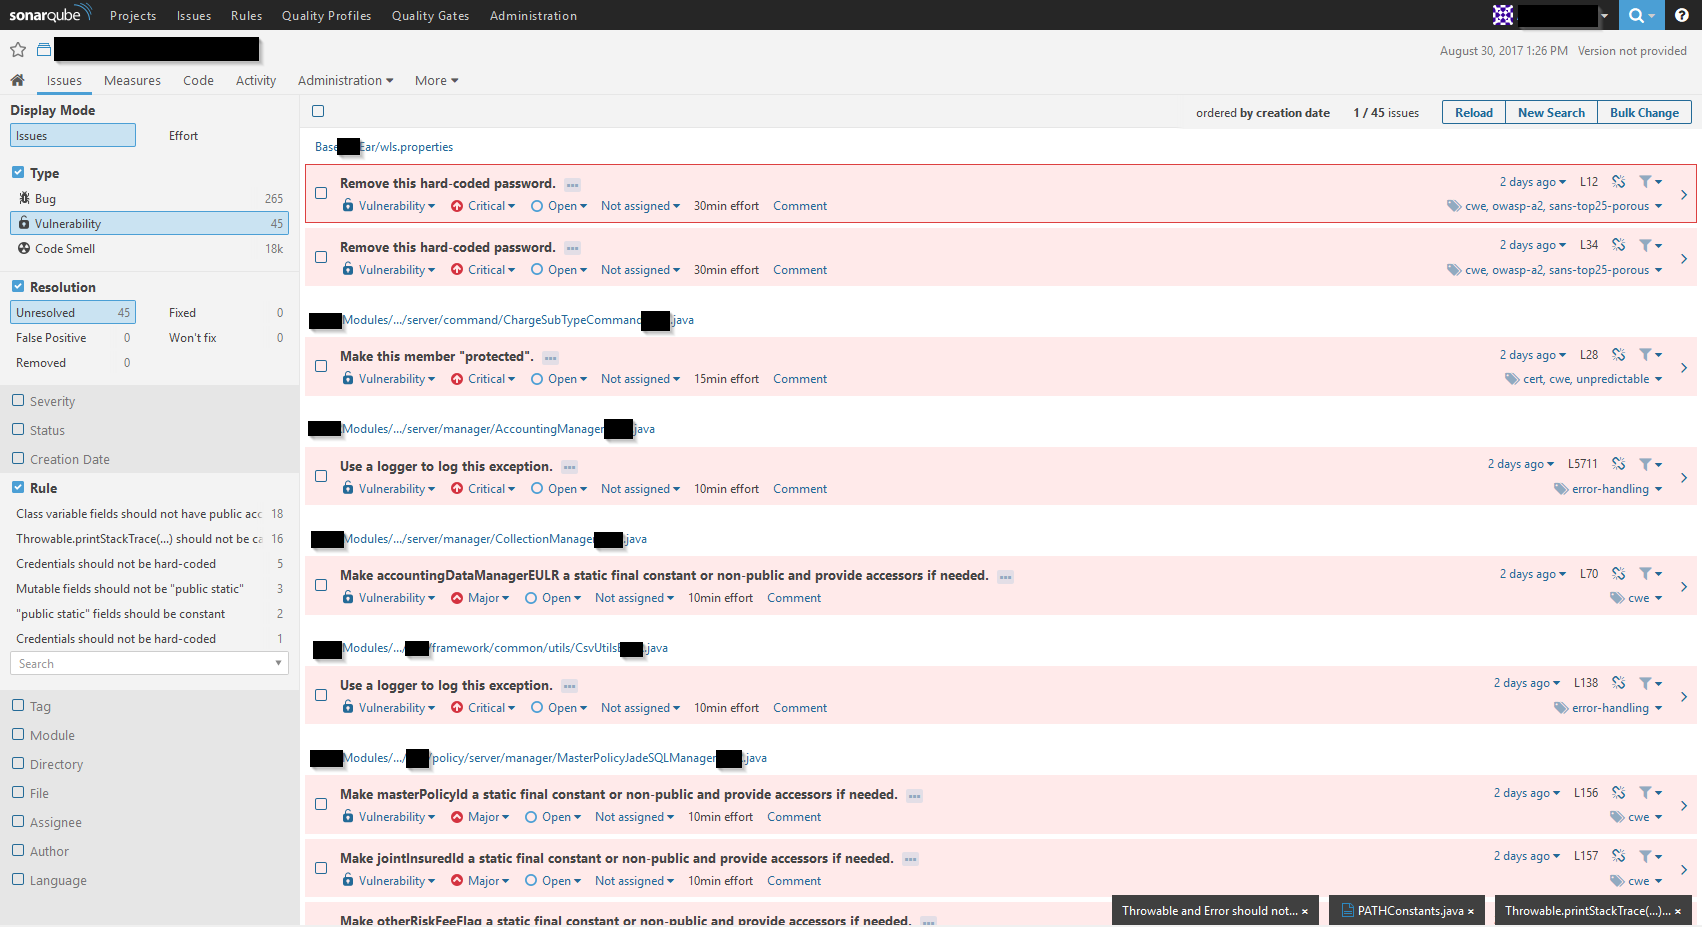
\includegraphics[width=\paperwidth]{images/sonar_sec_audit}}
	\caption{Extrait des résultats de sécurité du scanner Sonar}
	\label{fig:sonar_sec}
\end{figure}

C'est durant l'audit que j'ai majoritairement utilisé Sonar, mais les scripts de CI qui étaient en plus avant mon arrivée chez Alter Frame incorporaient déjà des analyses Sonar effectuées sur le code. C'est d'ailleurs de ce fait (mon tuteur ayant déjà de l'expérience avec ce logiciel) ainsi que du faible nombre de concurrents gratuits\cite{squale} que nous avons choisi d'utiliser Sonar dans ce cas de figure.

\subsubsection{JMeter \& SoapUI}
Ces deux outils, de même que ZAP, avaient déjà été utilisés lors des itérations précédentes de l'audit, et les conserver permettait de comparer facilement les résultats que nous obtiendrions avec les résultats antérieurs. Aussi, en l'absence de raison de ne \emph{pas} les conserver, nous les avons conservés.

SoapUI\cite{soapui} est un outil de test pour applications REST ou SOAP. L'application auditée utilisait le protocole SOAP, et SoapUI nous a servi à modifier et rejouer des requêtes isolées, sans tester les performances de l'application mais pour en saisir le fonctionnement et préparer le véritable test, en plus de vérifier que nous avions bien les droits pour réaliser toutes les opérations prévues.

JMeter est un outil de test de performances pour applications web en général. Le panel de fonctionnalités qu'il offre est extrêmement large (et en conséquence, sa prise en main est loin d'être triviale) et nous n'en avons utilisé qu'une partie : configurer JMeter comme proxy pour enregistrer un cas d'utilisation typique qui servira de scénario de test (on peut voir les différentes étapes d'un tel scénario dans l'interface de JMeter dans la figure~\ref{fig:jmeter}), puis rejouer celui-ci en boucle et plusieurs fois en parallèle pour tester les limites de l'application.
\begin{figure}
  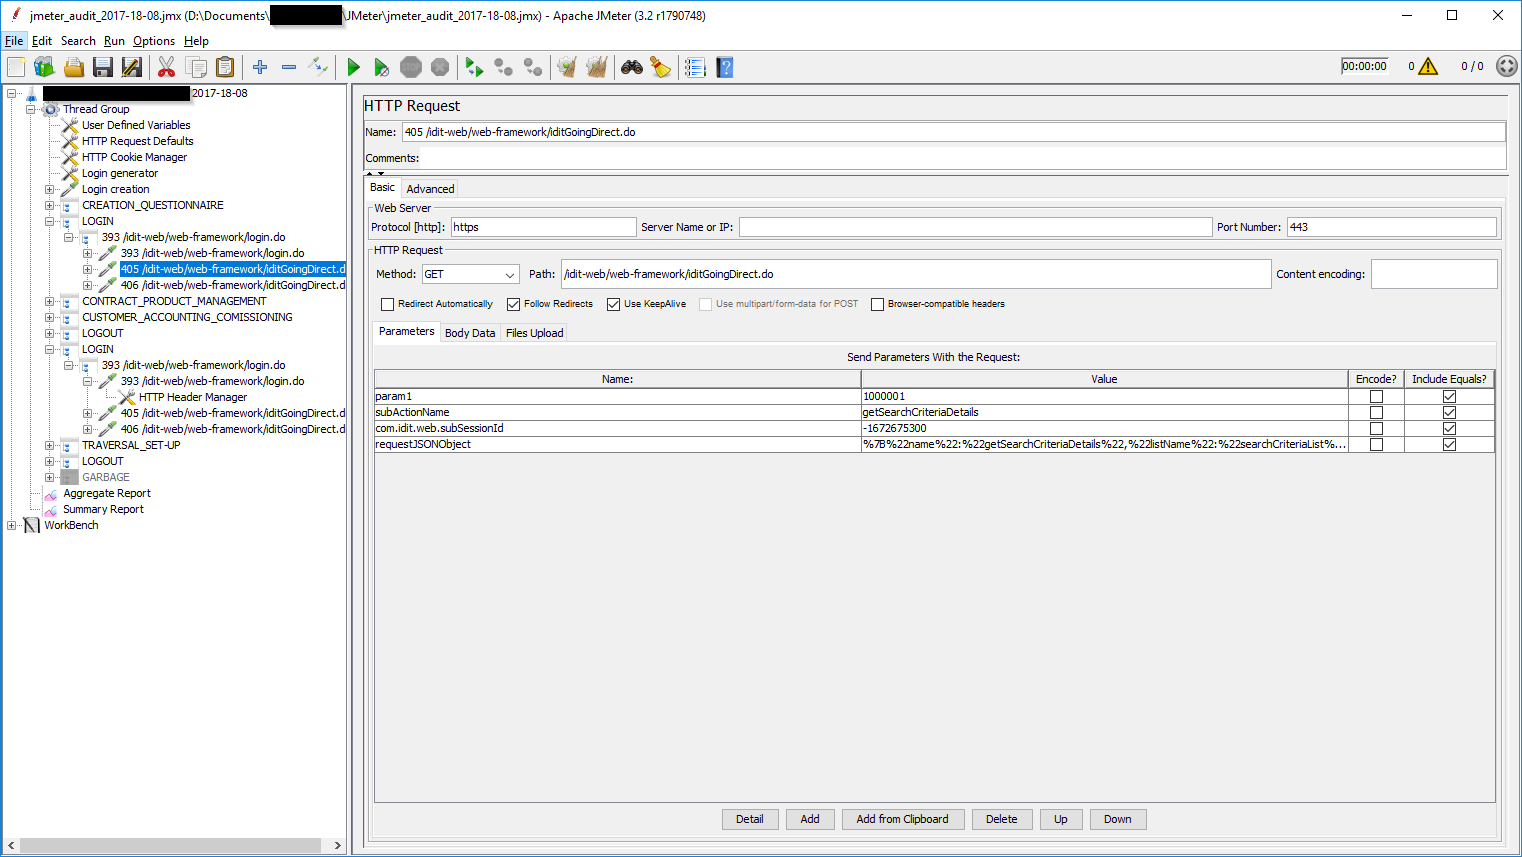
\includegraphics[width=\linewidth]{images/jmeter}
  \caption{JMeter, une fois configuré}
  \label{fig:jmeter}
\end{figure}

%TODO: ajouter un screen de JMeter
%%% Local Variables:
%%% mode: latex
%%% TeX-master: "../M2FSI-rapport-LEONARDI-alexandre"
%%% End:

\pagebreak
\section{Synthèse du travail effectué}

\pagebreak
\clearpage
\vspace*{\fill}
\begin{center}
\begin{minipage}{.6\textwidth}
\Huge Rapport technique
\end{minipage}
\end{center}
\vfill % equivalent to \vspace{\fill}
\clearpage
\pagebreak

\section{Sécurité \& intégration continue}
La seconde partie de mon stage a été majoritairement consacrée à l'amélioration
du processus de CI au sein d'Alter Frame 
\pagebreak
\section{Développement Java}
La pemière partie de mon stage a été occupé par beaucoup de développement en Java. L'idée de cette part du stage était de participer aux contrats remplis par Alter Frame et avoir ainsi une idée précise d'à quoi ressemblait le travail dans l'entreprise. Je vais profiter de cette partie pour résumer les projets auxquels j'ai participé et dans quelle mesure, sans pour autant le commanditaire dans un soucis de discrétion.

\subsection{Outil de gestion de tests pour un constructeur automobile}
\subsubsection{Le contexte}
Produire et mettre en vente une voiture requière que celle-ci soit passée par une batterie de tests intensifs. Ce premier projet était un logiciel permettant de gérer ces tests de bout en bout : ajouter un véhicule à la base de données, établir une liste d'organes à tester, une liste de tests pour chaque organe, puis ensuite enregistrer les résultats des tests qui ont été effectués. Cela représente le c\oe{}ur de la logique métier impliquée dans le logiciel, mais naturellement il y avait autour de ce noyau de nombreuses fonctionnalités plus ``classiques'' telles que la gestion d'authentification des utilisateurs, les différents privilèges (administrateur, utilisateur simple), etc.

De manière intéressante, j'ai remarqué en travaillant sur le workflow des tests automobile implémenté dans cet outil que celui-ci est semblable au cycle en V qui fait partie intégrante de la gestion de projet en informatique. Les détails étaient, naturellement, très différents mais ce qui semblait être les grandes lignes de la façon dont un projet de tests devait être géré était au contraire très proche de ce que nous connaissons dans le monde de l'informatique.

Une particularité de ce projet est qu'il s'agit d'un logiciel déjà existant qui a été récupéré par Alter Frame pour de la mise à jour et de la maintenance. L'ESN initialement en charge du projet avait perdu le contrat et mon travail a, de ce fait, été majoritairement constitué de correction de bugs et, dans une moindre mesure, d'ajout de fonctionnalités mineures (voir section~\ref{subsec:ajout}).

\subsubsection{Environnement technique}
TRANSFORMER CE QUI SUIT EN LISTE À POINTS !!
\subsubsection{Java 7}
Le projet étant vieux de plusieurs années déjà, il utilise la version de Java qui était en vigueur à l'époque de sa genèse à savoir Java 7.

\subsubsection{Java Swing}
Pour les mêmes raisons que Java 7, le framework utilisé pour la partie graphique de l'application est Java Swing\footnote{\url{https://fr.wikipedia.org/wiki/Swing_(Java)}}.

\subsubsection{ActiveMQ}

\subsubsection{Fonctionnalités ajoutées}
\label{subsec:ajout}
tmp

\pagebreak
\section{Audit de sécurité et de performances}
\label{sec:audit}
J'ai eu l'occasion, sur la fin de mon stage, de réaliser un audit pour une société travaillant dans le monde de l'assurance. Ce genre de projets sort du cadre habituel de ceux entrepris par Alter Frame. C'est un contrat historiquement entretenu par Alter Frame depuis plusieurs années, et une opportunité intéressante de s'éloigner du développement et de faire une mission de conseil. 

L'audit comportait trois axes importants : la qualité, la sécurité et la performance. 

\subsection{Méthodologie}
Mon intervention a naturellement concerné ces trois aspects, et ce de trois façons différentes. 

\subsubsection{Sécurité}
Il s'agit naturellement de la partie où mon intervention a été la plus notable (NOTE : est-ce que ça fait pas pompeux ?!!!). Les analyses de séurité se sont faites sur site, à partir d'une machine configurée par le client : l'intervention concerne une application web disponible uniquement en intranet chez le client et leurs procédures et protocoles de sécurité rendent très compliqué d'exporter l'appplication pour l'auditer à partir des locaux d'Alter Frame. 

Le test a consisté à mener des analyses avec OWASP ZAP et à analyser et rejouer les résultats, trier les faux positifs des vraies failles de sécurité et faire un état de l'évolution de l'application depuis le précédent audit qui date d'un an. 

Nous avons utilisé les fonctionnalités classiques de ZAP pour obtenir un résultat le plus exhaustif possible compte tenu du peu de temps alloué à l'audit de sécurité : d'abord \textit{spider} l'application cible pour que le proxy en découvre la majorité, avant de lancer un scan actif qui, compte tenu de la taille de l'application auditée, a pris plusieurs heures de temps d'exécution. 

Le test a également incorporé une partie audit de code, supportée par l'utilisation de SonarQube et qui se recoupera avec la partie qualité. Sonar peut, en effet, être configuré pour retourner des alertes de sécurité en ce qui concerne le code analysé. Comme pour ZAP il requière une intervention humaine pour écarter les faux positifs et n'offre aucune garantie d'exhaustivité, mais cela représentait un point d'entrée efficace pour chercher des traces de risques dans le code audité. 

\subsubsection{Performance}
La partie audit de performance a elle aussi compris deux sous parties, l'une dynamique basée sur l'utilisation de JMeter\footnote{\url{http://jmeter.apache.org/}} et de nmon\footnote{\url{http://nmon.sourceforge.net/pmwiki.php}}, l'autre statique (à savoir, une analyse de code). Je ne suis personellement intervenu que sur la partie dynamique qui s'est effectuée sur site pour les mêmes raisons que l'analyse de sécurité. 

JMeter est un outil développé par Apache qui permet de faire des tests de charge d'applications Web. Les fonctionnalités de l'outil sont impressionantes de diversité et de profondeur et comme encore une fois le temps alloué à l'auit était court, je n'ai pu qu'en effleurer la surface : mon travail a consisté à enregistrer une série de cas d'utilisation typiques en plaçant JMeter en proxy de navigation, puis à les configurer pour qu'ils soient reproductibles automatiquement (par exemple en générant des utilisateurs de manière procédurale) et à les rejouer en boucle. 

JMeter produit des résultats très complets formatés en HTML qui affichent plusieurs métriques sous formes de graphiques ou de tableaux récapitulatifs, et nous avons effectué plusieurs jeux de test en augmentant à chaque fois la charge à laquelle le serveur était soumis pour observser son comportement jusq'au point où il "tombe".

Nmon pour sa part est un outil de monitoring 

\subsubsection{}

\subsection{Résultats obtenus}

\pagebreak

\section*{Conclusion}

Penser à mettre les crédits pour le template
\pagebreak

%\bibliography{parts/biblio}
%\bibliographystyle{plainmat}

\end{document}
